\documentclass[1p]{elsarticle_modified}
%\bibliographystyle{elsarticle-num}

%\usepackage[colorlinks]{hyperref}
%\usepackage{abbrmath_seonhwa} %\Abb, \Ascr, \Acal ,\Abf, \Afrak
\usepackage{amsfonts}
\usepackage{amssymb}
\usepackage{amsmath}
\usepackage{amsthm}
\usepackage{scalefnt}
\usepackage{amsbsy}
\usepackage{kotex}
\usepackage{caption}
\usepackage{subfig}
\usepackage{color}
\usepackage{graphicx}
\usepackage{xcolor} %% white, black, red, green, blue, cyan, magenta, yellow
\usepackage{float}
\usepackage{setspace}
\usepackage{hyperref}

\usepackage{tikz}
\usetikzlibrary{arrows}

\usepackage{multirow}
\usepackage{array} % fixed length table
\usepackage{hhline}

%%%%%%%%%%%%%%%%%%%%%
\makeatletter
\renewcommand*\env@matrix[1][\arraystretch]{%
	\edef\arraystretch{#1}%
	\hskip -\arraycolsep
	\let\@ifnextchar\new@ifnextchar
	\array{*\c@MaxMatrixCols c}}
\makeatother %https://tex.stackexchange.com/questions/14071/how-can-i-increase-the-line-spacing-in-a-matrix
%%%%%%%%%%%%%%%

\usepackage[normalem]{ulem}

\newcommand{\msout}[1]{\ifmmode\text{\sout{\ensuremath{#1}}}\else\sout{#1}\fi}
%SOURCE: \msout is \stkout macro in https://tex.stackexchange.com/questions/20609/strikeout-in-math-mode

\newcommand{\cancel}[1]{
	\ifmmode
	{\color{red}\msout{#1}}
	\else
	{\color{red}\sout{#1}}
	\fi
}

\newcommand{\add}[1]{
	{\color{blue}\uwave{#1}}
}

\newcommand{\replace}[2]{
	\ifmmode
	{\color{red}\msout{#1}}{\color{blue}\uwave{#2}}
	\else
	{\color{red}\sout{#1}}{\color{blue}\uwave{#2}}
	\fi
}

\newcommand{\Sol}{\mathcal{S}} %segment
\newcommand{\D}{D} %diagram
\newcommand{\A}{\mathcal{A}} %arc


%%%%%%%%%%%%%%%%%%%%%%%%%%%%%5 test

\def\sl{\operatorname{\textup{SL}}(2,\Cbb)}
\def\psl{\operatorname{\textup{PSL}}(2,\Cbb)}
\def\quan{\mkern 1mu \triangleright \mkern 1mu}

\theoremstyle{definition}
\newtheorem{thm}{Theorem}[section]
\newtheorem{prop}[thm]{Proposition}
\newtheorem{lem}[thm]{Lemma}
\newtheorem{ques}[thm]{Question}
\newtheorem{cor}[thm]{Corollary}
\newtheorem{defn}[thm]{Definition}
\newtheorem{exam}[thm]{Example}
\newtheorem{rmk}[thm]{Remark}
\newtheorem{alg}[thm]{Algorithm}

\newcommand{\I}{\sqrt{-1}}
\begin{document}

%\begin{frontmatter}
%
%\title{Boundary parabolic representations of knots up to 8 crossings}
%
%%% Group authors per affiliation:
%\author{Yunhi Cho} 
%\address{Department of Mathematics, University of Seoul, Seoul, Korea}
%\ead{yhcho@uos.ac.kr}
%
%
%\author{Seonhwa Kim} %\fnref{s_kim}}
%\address{Center for Geometry and Physics, Institute for Basic Science, Pohang, 37673, Korea}
%\ead{ryeona17@ibs.re.kr}
%
%\author{Hyuk Kim}
%\address{Department of Mathematical Sciences, Seoul National University, Seoul 08826, Korea}
%\ead{hyukkim@snu.ac.kr}
%
%\author{Seokbeom Yoon}
%\address{Department of Mathematical Sciences, Seoul National University, Seoul, 08826,  Korea}
%\ead{sbyoon15@snu.ac.kr}
%
%\begin{abstract}
%We find all boundary parabolic representation of knots up to 8 crossings.
%
%\end{abstract}
%\begin{keyword}
%    \MSC[2010] 57M25 
%\end{keyword}
%
%\end{frontmatter}

%\linenumbers
%\tableofcontents
%
\newcommand\colored[1]{\textcolor{white}{\rule[-0.35ex]{0.8em}{1.4ex}}\kern-0.8em\color{red} #1}%
%\newcommand\colored[1]{\textcolor{white}{ #1}\kern-2.17ex	\textcolor{white}{ #1}\kern-1.81ex	\textcolor{white}{ #1}\kern-2.15ex\color{red}#1	}

{\Large $\underline{12n_{0651}~(K12n_{0651})}$}

\setlength{\tabcolsep}{10pt}
\renewcommand{\arraystretch}{1.6}
\vspace{1cm}\begin{tabular}{m{100pt}>{\centering\arraybackslash}m{274pt}}
\multirow{5}{120pt}{
	\centering
	\includegraphics[width=112pt]{../../../GIT/diagram.site/Diagrams/png/2740_12n_0651.png}\\
\ \ \ A knot diagram\footnotemark}&
\allowdisplaybreaks
\textbf{Linearized knot diagam} \\
\cline{2-2}
 &
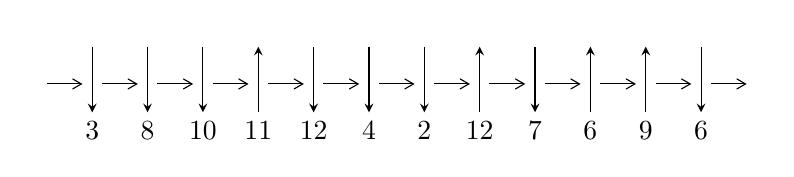
\begin{tikzpicture}[x=20pt, y=17pt]
	% nodes
	\node (C0) at (0, 0) {};
	\node (C1) at (1, 0) {};
	\node (C1U) at (1, +1) {};
	\node (C1D) at (1, -1) {3};

	\node (C2) at (2, 0) {};
	\node (C2U) at (2, +1) {};
	\node (C2D) at (2, -1) {8};

	\node (C3) at (3, 0) {};
	\node (C3U) at (3, +1) {};
	\node (C3D) at (3, -1) {10};

	\node (C4) at (4, 0) {};
	\node (C4U) at (4, +1) {};
	\node (C4D) at (4, -1) {11};

	\node (C5) at (5, 0) {};
	\node (C5U) at (5, +1) {};
	\node (C5D) at (5, -1) {12};

	\node (C6) at (6, 0) {};
	\node (C6U) at (6, +1) {};
	\node (C6D) at (6, -1) {4};

	\node (C7) at (7, 0) {};
	\node (C7U) at (7, +1) {};
	\node (C7D) at (7, -1) {2};

	\node (C8) at (8, 0) {};
	\node (C8U) at (8, +1) {};
	\node (C8D) at (8, -1) {12};

	\node (C9) at (9, 0) {};
	\node (C9U) at (9, +1) {};
	\node (C9D) at (9, -1) {7};

	\node (C10) at (10, 0) {};
	\node (C10U) at (10, +1) {};
	\node (C10D) at (10, -1) {6};

	\node (C11) at (11, 0) {};
	\node (C11U) at (11, +1) {};
	\node (C11D) at (11, -1) {9};

	\node (C12) at (12, 0) {};
	\node (C12U) at (12, +1) {};
	\node (C12D) at (12, -1) {6};
	\node (C13) at (13, 0) {};

	% arrows
	\draw[->,>={angle 60}]
	(C0) edge (C1) (C1) edge (C2) (C2) edge (C3) (C3) edge (C4) (C4) edge (C5) (C5) edge (C6) (C6) edge (C7) (C7) edge (C8) (C8) edge (C9) (C9) edge (C10) (C10) edge (C11) (C11) edge (C12) (C12) edge (C13) ;	\draw[->,>=stealth]
	(C1U) edge (C1D) (C2U) edge (C2D) (C3U) edge (C3D) (C4D) edge (C4U) (C5U) edge (C5D) (C6U) edge (C6D) (C7U) edge (C7D) (C8D) edge (C8U) (C9U) edge (C9D) (C10D) edge (C10U) (C11D) edge (C11U) (C12U) edge (C12D) ;
	\end{tikzpicture} \\
\hhline{~~} \\& 
\textbf{Solving Sequence} \\ \cline{2-2} 
 &
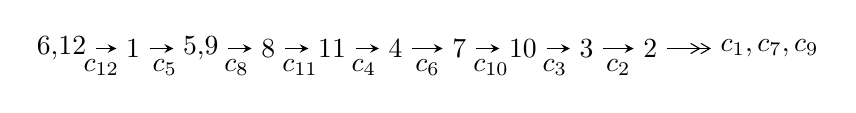
\begin{tikzpicture}[x=23pt, y=7pt]
	% node
	\node (A0) at (-1/8, 0) {6,12};
	\node (A1) at (1, 0) {1};
	\node (A2) at (33/16, 0) {5,9};
	\node (A3) at (25/8, 0) {8};
	\node (A4) at (33/8, 0) {11};
	\node (A5) at (41/8, 0) {4};
	\node (A6) at (49/8, 0) {7};
	\node (A7) at (57/8, 0) {10};
	\node (A8) at (65/8, 0) {3};
	\node (A9) at (73/8, 0) {2};
	\node (C1) at (1/2, -1) {$c_{12}$};
	\node (C2) at (3/2, -1) {$c_{5}$};
	\node (C3) at (21/8, -1) {$c_{8}$};
	\node (C4) at (29/8, -1) {$c_{11}$};
	\node (C5) at (37/8, -1) {$c_{4}$};
	\node (C6) at (45/8, -1) {$c_{6}$};
	\node (C7) at (53/8, -1) {$c_{10}$};
	\node (C8) at (61/8, -1) {$c_{3}$};
	\node (C9) at (69/8, -1) {$c_{2}$};
	\node (A10) at (11, 0) {$c_{1},c_{7},c_{9}$};

	% edge
	\draw[->,>=stealth]	
	(A0) edge (A1) (A1) edge (A2) (A2) edge (A3) (A3) edge (A4) (A4) edge (A5) (A5) edge (A6) (A6) edge (A7) (A7) edge (A8) (A8) edge (A9) ;
	\draw[->>,>={angle 60}]	
	(A9) edge (A10);
\end{tikzpicture} \\ 

\end{tabular} \\

\footnotetext{
The image of knot diagram is generated by the software ``\textbf{Draw programme}" developed by Andrew Bartholomew(\url{http://www.layer8.co.uk/maths/draw/index.htm\#Running-draw}), where we modified some parts for our purpose(\url{https://github.com/CATsTAILs/LinksPainter}).
}\phantom \\ \newline 
\centering \textbf{Ideals for irreducible components\footnotemark of $X_{\text{par}}$} 
 
\begin{align*}
I^u_{1}&=\langle 
-5.87738\times10^{79} u^{37}-4.81123\times10^{79} u^{36}+\cdots+1.09631\times10^{80} b+6.40170\times10^{79},\\
\phantom{I^u_{1}}&\phantom{= \langle  }-5.87738\times10^{79} u^{37}-4.81123\times10^{79} u^{36}+\cdots+1.09631\times10^{80} a-4.56137\times10^{79},\;u^{38}+u^{37}+\cdots-2 u+1\rangle \\
I^u_{2}&=\langle 
-1.04653\times10^{27} u^{29}+6.40175\times10^{26} u^{28}+\cdots+7.20755\times10^{25} b-2.20858\times10^{27},\\
\phantom{I^u_{2}}&\phantom{= \langle  }-1.04653\times10^{27} u^{29}+6.40175\times10^{26} u^{28}+\cdots+7.20755\times10^{25} a-2.13651\times10^{27},\;u^{30}+u^{28}+\cdots+2 u+1\rangle \\
I^u_{3}&=\langle 
-8.10037\times10^{37} u^{23}-8.29349\times10^{37} u^{22}+\cdots+3.72935\times10^{40} b+3.34631\times10^{39},\\
\phantom{I^u_{3}}&\phantom{= \langle  }-4.67951\times10^{43} u^{23}-5.81164\times10^{43} u^{22}+\cdots+3.64130\times10^{45} a+6.70319\times10^{45},\\
\phantom{I^u_{3}}&\phantom{= \langle  }u^{24}+u^{23}+\cdots-72 u+389\rangle \\
I^u_{4}&=\langle 
-7.05840\times10^{36} u^{23}+1.01927\times10^{37} u^{22}+\cdots+1.33403\times10^{40} b-9.50718\times10^{39},\\
\phantom{I^u_{4}}&\phantom{= \langle  }-4.57492\times10^{42} u^{23}+4.23759\times10^{42} u^{22}+\cdots+2.64466\times10^{45} a-1.17455\times10^{45},\\
\phantom{I^u_{4}}&\phantom{= \langle  }u^{24}+12 u^{22}+\cdots+1224 u+631\rangle \\
I^u_{5}&=\langle 
b,\;a-1,\;u^3- u^2+2 u-1\rangle \\
\\
\end{align*}
\raggedright * 5 irreducible components of $\dim_{\mathbb{C}}=0$, with total 119 representations.\\
\footnotetext{All coefficients of polynomials are rational numbers. But the coefficients are sometimes approximated in decimal forms when there is not enough margin.}
\newpage
\renewcommand{\arraystretch}{1}
\centering \section*{I. $I^u_{1}= \langle -5.88\times10^{79} u^{37}-4.81\times10^{79} u^{36}+\cdots+1.10\times10^{80} b+6.40\times10^{79},\;-5.88\times10^{79} u^{37}-4.81\times10^{79} u^{36}+\cdots+1.10\times10^{80} a-4.56\times10^{79},\;u^{38}+u^{37}+\cdots-2 u+1 \rangle$}
\flushleft \textbf{(i) Arc colorings}\\
\begin{tabular}{m{7pt} m{180pt} m{7pt} m{180pt} }
\flushright $a_{6}=$&$\begin{pmatrix}0\\u\end{pmatrix}$ \\
\flushright $a_{12}=$&$\begin{pmatrix}1\\0\end{pmatrix}$ \\
\flushright $a_{1}=$&$\begin{pmatrix}1\\u^2\end{pmatrix}$ \\
\flushright $a_{5}=$&$\begin{pmatrix}u\\u\end{pmatrix}$ \\
\flushright $a_{9}=$&$\begin{pmatrix}0.536107 u^{37}+0.438858 u^{36}+\cdots+5.20206 u+0.416067\\0.536107 u^{37}+0.438858 u^{36}+\cdots+5.20206 u-0.583933\end{pmatrix}$ \\
\flushright $a_{8}=$&$\begin{pmatrix}1\\0.536107 u^{37}+0.438858 u^{36}+\cdots+5.20206 u-0.583933\end{pmatrix}$ \\
\flushright $a_{11}=$&$\begin{pmatrix}0.551933 u^{37}+0.184165 u^{36}+\cdots+5.75746 u-1.74427\\0.0158259 u^{37}-0.254694 u^{36}+\cdots+0.555407 u-2.16033\end{pmatrix}$ \\
\flushright $a_{4}=$&$\begin{pmatrix}0.880326 u^{37}+1.05073 u^{36}+\cdots+6.21709 u-0.512405\\0.415309 u^{37}+0.344712 u^{36}+\cdots+6.06497 u-1.60045\end{pmatrix}$ \\
\flushright $a_{7}=$&$\begin{pmatrix}0.370131 u^{37}+0.566178 u^{36}+\cdots+2.00968 u+1.02387\\0.484697 u^{37}+0.579181 u^{36}+\cdots+5.16811 u-0.0626616\end{pmatrix}$ \\
\flushright $a_{10}=$&$\begin{pmatrix}0.551933 u^{37}+0.184165 u^{36}+\cdots+5.75746 u-1.74427\\-0.138322 u^{37}-0.383483 u^{36}+\cdots-0.732063 u-1.79256\end{pmatrix}$ \\
\flushright $a_{3}=$&$\begin{pmatrix}-0.603900 u^{37}-0.605524 u^{36}+\cdots-4.99750 u+1.42841\\-0.121286 u^{37}+0.101025 u^{36}+\cdots-2.38717 u+2.45390\end{pmatrix}$ \\
\flushright $a_{2}=$&$\begin{pmatrix}-0.624236 u^{37}-0.742981 u^{36}+\cdots-4.51871 u-0.410519\\-0.794152 u^{37}-0.640181 u^{36}+\cdots-8.11717 u+1.88051\end{pmatrix}$\\&\end{tabular}
\flushleft \textbf{(ii) Obstruction class $= -1$}\\~\\
\flushleft \textbf{(iii) Cusp Shapes $= -1.67858 u^{37}-0.851719 u^{36}+\cdots-22.0981 u+8.20713$}\\~\\
\newpage\renewcommand{\arraystretch}{1}
\flushleft \textbf{(iv) u-Polynomials at the component}\newline \\
\begin{tabular}{m{50pt}|m{274pt}}
Crossings & \hspace{64pt}u-Polynomials at each crossing \\
\hline $$\begin{aligned}c_{1}\end{aligned}$$&$\begin{aligned}
&u^{38}+20 u^{37}+\cdots+65536 u+65536
\end{aligned}$\\
\hline $$\begin{aligned}c_{2},c_{7}\end{aligned}$$&$\begin{aligned}
&u^{38}-16 u^{37}+\cdots-2560 u+256
\end{aligned}$\\
\hline $$\begin{aligned}c_{3},c_{9}\end{aligned}$$&$\begin{aligned}
&u^{38}-2 u^{37}+\cdots-8 u+1
\end{aligned}$\\
\hline $$\begin{aligned}c_{4}\end{aligned}$$&$\begin{aligned}
&u^{38}-22 u^{36}+\cdots-1528 u+1456
\end{aligned}$\\
\hline $$\begin{aligned}c_{5},c_{12}\end{aligned}$$&$\begin{aligned}
&u^{38}- u^{37}+\cdots+2 u+1
\end{aligned}$\\
\hline $$\begin{aligned}c_{6}\end{aligned}$$&$\begin{aligned}
&u^{38}-19 u^{37}+\cdots-3108 u+245
\end{aligned}$\\
\hline $$\begin{aligned}c_{8},c_{11}\end{aligned}$$&$\begin{aligned}
&u^{38}+12 u^{37}+\cdots+1309 u+245
\end{aligned}$\\
\hline $$\begin{aligned}c_{10}\end{aligned}$$&$\begin{aligned}
&u^{38}- u^{37}+\cdots-189 u+61
\end{aligned}$\\
\hline
\end{tabular}\\~\\
\newpage\renewcommand{\arraystretch}{1}
\flushleft \textbf{(v) Riley Polynomials at the component}\newline \\
\begin{tabular}{m{50pt}|m{274pt}}
Crossings & \hspace{64pt}Riley Polynomials at each crossing \\
\hline $$\begin{aligned}c_{1}\end{aligned}$$&$\begin{aligned}
&y^{38}-4 y^{37}+\cdots-15032385536 y+4294967296
\end{aligned}$\\
\hline $$\begin{aligned}c_{2},c_{7}\end{aligned}$$&$\begin{aligned}
&y^{38}-20 y^{37}+\cdots-65536 y+65536
\end{aligned}$\\
\hline $$\begin{aligned}c_{3},c_{9}\end{aligned}$$&$\begin{aligned}
&y^{38}+20 y^{37}+\cdots+38 y+1
\end{aligned}$\\
\hline $$\begin{aligned}c_{4}\end{aligned}$$&$\begin{aligned}
&y^{38}-44 y^{37}+\cdots-18656544 y+2119936
\end{aligned}$\\
\hline $$\begin{aligned}c_{5},c_{12}\end{aligned}$$&$\begin{aligned}
&y^{38}+51 y^{37}+\cdots+14 y+1
\end{aligned}$\\
\hline $$\begin{aligned}c_{6}\end{aligned}$$&$\begin{aligned}
&y^{38}-9 y^{37}+\cdots+500486 y+60025
\end{aligned}$\\
\hline $$\begin{aligned}c_{8},c_{11}\end{aligned}$$&$\begin{aligned}
&y^{38}+12 y^{37}+\cdots+698299 y+60025
\end{aligned}$\\
\hline $$\begin{aligned}c_{10}\end{aligned}$$&$\begin{aligned}
&y^{38}-27 y^{37}+\cdots-45603 y+3721
\end{aligned}$\\
\hline
\end{tabular}\\~\\
\newpage\flushleft \textbf{(vi) Complex Volumes and Cusp Shapes}
$$\begin{array}{c|c|c}  
\text{Solutions to }I^u_{1}& \I (\text{vol} + \sqrt{-1}CS) & \text{Cusp shape}\\
 \hline 
\begin{aligned}
u &= \phantom{-}0.769678 + 0.293616 I \\
a &= \phantom{-}0.990107 + 0.482059 I \\
b &= -0.009893 + 0.482059 I\end{aligned}
 & -1.363000 - 0.273225 I & -9.42966 + 1.77588 I \\ \hline\begin{aligned}
u &= \phantom{-}0.769678 - 0.293616 I \\
a &= \phantom{-}0.990107 - 0.482059 I \\
b &= -0.009893 - 0.482059 I\end{aligned}
 & -1.363000 + 0.273225 I & -9.42966 - 1.77588 I \\ \hline\begin{aligned}
u &= \phantom{-}0.145322 + 0.514446 I \\
a &= \phantom{-}0.88401 + 1.27389 I \\
b &= -0.115995 + 1.273890 I\end{aligned}
 & -5.36598 - 0.46970 I & -5.55031 + 3.34064 I \\ \hline\begin{aligned}
u &= \phantom{-}0.145322 - 0.514446 I \\
a &= \phantom{-}0.88401 - 1.27389 I \\
b &= -0.115995 - 1.273890 I\end{aligned}
 & -5.36598 + 0.46970 I & -5.55031 - 3.34064 I \\ \hline\begin{aligned}
u &= -0.471950 + 0.049779 I \\
a &= \phantom{-}1.55201 - 0.71853 I \\
b &= \phantom{-}0.552008 - 0.718532 I\end{aligned}
 & \phantom{-}0.91968 - 1.81363 I & -0.50505 + 3.48218 I \\ \hline\begin{aligned}
u &= -0.471950 - 0.049779 I \\
a &= \phantom{-}1.55201 + 0.71853 I \\
b &= \phantom{-}0.552008 + 0.718532 I\end{aligned}
 & \phantom{-}0.91968 + 1.81363 I & -0.50505 - 3.48218 I \\ \hline\begin{aligned}
u &= \phantom{-}0.451414 + 0.116571 I \\
a &= \phantom{-}1.47086 - 1.11033 I \\
b &= \phantom{-}0.470864 - 1.110330 I\end{aligned}
 & -1.87643 - 5.76844 I & -7.26109 + 7.17876 I \\ \hline\begin{aligned}
u &= \phantom{-}0.451414 - 0.116571 I \\
a &= \phantom{-}1.47086 + 1.11033 I \\
b &= \phantom{-}0.470864 + 1.110330 I\end{aligned}
 & -1.87643 + 5.76844 I & -7.26109 - 7.17876 I \\ \hline\begin{aligned}
u &= -1.52338 + 0.33853 I \\
a &= \phantom{-}0.660164 - 0.721621 I \\
b &= -0.339836 - 0.721621 I\end{aligned}
 & -9.11191 + 1.39764 I & \phantom{-0.000000 } 0 \\ \hline\begin{aligned}
u &= -1.52338 - 0.33853 I \\
a &= \phantom{-}0.660164 + 0.721621 I \\
b &= -0.339836 + 0.721621 I\end{aligned}
 & -9.11191 - 1.39764 I & \phantom{-0.000000 } 0\\
 \hline 
 \end{array}$$\newpage$$\begin{array}{c|c|c}  
\text{Solutions to }I^u_{1}& \I (\text{vol} + \sqrt{-1}CS) & \text{Cusp shape}\\
 \hline 
\begin{aligned}
u &= \phantom{-}0.41128 + 1.51296 I \\
a &= \phantom{-}0.046743 + 0.690253 I \\
b &= -0.953257 + 0.690253 I\end{aligned}
 & \phantom{-}1.47310 + 1.34582 I & \phantom{-0.000000 } 0 \\ \hline\begin{aligned}
u &= \phantom{-}0.41128 - 1.51296 I \\
a &= \phantom{-}0.046743 - 0.690253 I \\
b &= -0.953257 - 0.690253 I\end{aligned}
 & \phantom{-}1.47310 - 1.34582 I & \phantom{-0.000000 } 0 \\ \hline\begin{aligned}
u &= -0.016686 + 0.398344 I \\
a &= \phantom{-}1.31541 - 1.24871 I \\
b &= \phantom{-}0.315412 - 1.248710 I\end{aligned}
 & -1.19389 - 3.34823 I & \phantom{-}1.04129 + 3.46922 I \\ \hline\begin{aligned}
u &= -0.016686 - 0.398344 I \\
a &= \phantom{-}1.31541 + 1.24871 I \\
b &= \phantom{-}0.315412 + 1.248710 I\end{aligned}
 & -1.19389 + 3.34823 I & \phantom{-}1.04129 - 3.46922 I \\ \hline\begin{aligned}
u &= -0.310405 + 0.170863 I \\
a &= \phantom{-}1.95426 - 0.20841 I \\
b &= \phantom{-}0.954255 - 0.208414 I\end{aligned}
 & \phantom{-}2.29409 - 1.35414 I & \phantom{-}2.68942 + 3.98636 I \\ \hline\begin{aligned}
u &= -0.310405 - 0.170863 I \\
a &= \phantom{-}1.95426 + 0.20841 I \\
b &= \phantom{-}0.954255 + 0.208414 I\end{aligned}
 & \phantom{-}2.29409 + 1.35414 I & \phantom{-}2.68942 - 3.98636 I \\ \hline\begin{aligned}
u &= -0.19463 + 1.64159 I \\
a &= \phantom{-}0.195587 - 1.105580 I \\
b &= -0.804413 - 1.105580 I\end{aligned}
 & \phantom{-}0.19003 + 7.83950 I & \phantom{-0.000000 } 0 \\ \hline\begin{aligned}
u &= -0.19463 - 1.64159 I \\
a &= \phantom{-}0.195587 + 1.105580 I \\
b &= -0.804413 + 1.105580 I\end{aligned}
 & \phantom{-}0.19003 - 7.83950 I & \phantom{-0.000000 } 0 \\ \hline\begin{aligned}
u &= \phantom{-}0.230980 + 0.257221 I \\
a &= \phantom{-}1.92353 - 0.29790 I \\
b &= \phantom{-}0.923530 - 0.297905 I\end{aligned}
 & \phantom{-}1.90925 - 2.85593 I & -1.44584 + 3.55066 I \\ \hline\begin{aligned}
u &= \phantom{-}0.230980 - 0.257221 I \\
a &= \phantom{-}1.92353 + 0.29790 I \\
b &= \phantom{-}0.923530 + 0.297905 I\end{aligned}
 & \phantom{-}1.90925 + 2.85593 I & -1.44584 - 3.55066 I\\
 \hline 
 \end{array}$$\newpage$$\begin{array}{c|c|c}  
\text{Solutions to }I^u_{1}& \I (\text{vol} + \sqrt{-1}CS) & \text{Cusp shape}\\
 \hline 
\begin{aligned}
u &= \phantom{-}0.063281 + 0.328463 I \\
a &= \phantom{-}1.38439 + 1.55227 I \\
b &= \phantom{-}0.38439 + 1.55227 I\end{aligned}
 & -4.17774 + 8.19316 I & \phantom{-}2.57658 - 7.35106 I \\ \hline\begin{aligned}
u &= \phantom{-}0.063281 - 0.328463 I \\
a &= \phantom{-}1.38439 - 1.55227 I \\
b &= \phantom{-}0.38439 - 1.55227 I\end{aligned}
 & -4.17774 - 8.19316 I & \phantom{-}2.57658 + 7.35106 I \\ \hline\begin{aligned}
u &= -0.29571 + 1.65878 I \\
a &= -0.115023 + 0.852244 I \\
b &= -1.115020 + 0.852244 I\end{aligned}
 & \phantom{-}7.44352 + 10.43800 I & \phantom{-0.000000 } 0 \\ \hline\begin{aligned}
u &= -0.29571 - 1.65878 I \\
a &= -0.115023 - 0.852244 I \\
b &= -1.115020 - 0.852244 I\end{aligned}
 & \phantom{-}7.44352 - 10.43800 I & \phantom{-0.000000 } 0 \\ \hline\begin{aligned}
u &= \phantom{-}0.33699 + 1.67811 I \\
a &= \phantom{-}0.190397 - 0.903287 I \\
b &= -0.809603 - 0.903287 I\end{aligned}
 & \phantom{-}6.17744 - 3.28622 I & \phantom{-0.000000 } 0 \\ \hline\begin{aligned}
u &= \phantom{-}0.33699 - 1.67811 I \\
a &= \phantom{-}0.190397 + 0.903287 I \\
b &= -0.809603 + 0.903287 I\end{aligned}
 & \phantom{-}6.17744 + 3.28622 I & \phantom{-0.000000 } 0 \\ \hline\begin{aligned}
u &= \phantom{-}0.08401 + 1.79386 I \\
a &= -0.064653 - 0.833573 I \\
b &= -1.064650 - 0.833573 I\end{aligned}
 & \phantom{-}9.31632 - 4.00848 I & \phantom{-0.000000 } 0 \\ \hline\begin{aligned}
u &= \phantom{-}0.08401 - 1.79386 I \\
a &= -0.064653 + 0.833573 I \\
b &= -1.064650 + 0.833573 I\end{aligned}
 & \phantom{-}9.31632 + 4.00848 I & \phantom{-0.000000 } 0 \\ \hline\begin{aligned}
u &= -0.14610 + 1.84614 I \\
a &= \phantom{-}0.181975 + 0.975853 I \\
b &= -0.818025 + 0.975853 I\end{aligned}
 & \phantom{-}8.09306 - 3.65630 I & \phantom{-0.000000 } 0 \\ \hline\begin{aligned}
u &= -0.14610 - 1.84614 I \\
a &= \phantom{-}0.181975 - 0.975853 I \\
b &= -0.818025 - 0.975853 I\end{aligned}
 & \phantom{-}8.09306 + 3.65630 I & \phantom{-0.000000 } 0\\
 \hline 
 \end{array}$$\newpage$$\begin{array}{c|c|c}  
\text{Solutions to }I^u_{1}& \I (\text{vol} + \sqrt{-1}CS) & \text{Cusp shape}\\
 \hline 
\begin{aligned}
u &= -0.83573 + 1.82057 I \\
a &= \phantom{-}0.065993 - 1.107020 I \\
b &= -0.93401 - 1.10702 I\end{aligned}
 & \phantom{-}6.5788 + 17.8341 I & \phantom{-0.000000 } 0 \\ \hline\begin{aligned}
u &= -0.83573 - 1.82057 I \\
a &= \phantom{-}0.065993 + 1.107020 I \\
b &= -0.93401 + 1.10702 I\end{aligned}
 & \phantom{-}6.5788 - 17.8341 I & \phantom{-0.000000 } 0 \\ \hline\begin{aligned}
u &= -0.69403 + 1.88222 I \\
a &= \phantom{-}0.117388 - 0.861621 I \\
b &= -0.882612 - 0.861621 I\end{aligned}
 & \phantom{-}8.47233 + 2.68142 I & \phantom{-0.000000 } 0 \\ \hline\begin{aligned}
u &= -0.69403 - 1.88222 I \\
a &= \phantom{-}0.117388 + 0.861621 I \\
b &= -0.882612 + 0.861621 I\end{aligned}
 & \phantom{-}8.47233 - 2.68142 I & \phantom{-0.000000 } 0 \\ \hline\begin{aligned}
u &= \phantom{-}0.61560 + 1.91074 I \\
a &= \phantom{-}0.092836 + 1.092150 I \\
b &= -0.90716 + 1.09215 I\end{aligned}
 & \phantom{-}8.46080 - 11.17390 I & \phantom{-0.000000 } 0 \\ \hline\begin{aligned}
u &= \phantom{-}0.61560 - 1.91074 I \\
a &= \phantom{-}0.092836 - 1.092150 I \\
b &= -0.90716 - 1.09215 I\end{aligned}
 & \phantom{-}8.46080 + 11.17390 I & \phantom{-0.000000 } 0 \\ \hline\begin{aligned}
u &= \phantom{-}0.88007 + 1.80431 I \\
a &= \phantom{-}0.154018 + 0.915742 I \\
b &= -0.845982 + 0.915742 I\end{aligned}
 & \phantom{-}6.17371 - 9.49223 I & \phantom{-0.000000 } 0 \\ \hline\begin{aligned}
u &= \phantom{-}0.88007 - 1.80431 I \\
a &= \phantom{-}0.154018 - 0.915742 I \\
b &= -0.845982 - 0.915742 I\end{aligned}
 & \phantom{-}6.17371 + 9.49223 I & \phantom{-0.000000 } 0\\
 \hline 
 \end{array}$$\newpage\newpage\renewcommand{\arraystretch}{1}
\centering \section*{II. $I^u_{2}= \langle -1.05\times10^{27} u^{29}+6.40\times10^{26} u^{28}+\cdots+7.21\times10^{25} b-2.21\times10^{27},\;-1.05\times10^{27} u^{29}+6.40\times10^{26} u^{28}+\cdots+7.21\times10^{25} a-2.14\times10^{27},\;u^{30}+u^{28}+\cdots+2 u+1 \rangle$}
\flushleft \textbf{(i) Arc colorings}\\
\begin{tabular}{m{7pt} m{180pt} m{7pt} m{180pt} }
\flushright $a_{6}=$&$\begin{pmatrix}0\\u\end{pmatrix}$ \\
\flushright $a_{12}=$&$\begin{pmatrix}1\\0\end{pmatrix}$ \\
\flushright $a_{1}=$&$\begin{pmatrix}1\\u^2\end{pmatrix}$ \\
\flushright $a_{5}=$&$\begin{pmatrix}u\\u\end{pmatrix}$ \\
\flushright $a_{9}=$&$\begin{pmatrix}14.5199 u^{29}-8.88201 u^{28}+\cdots+8.39444 u+29.6427\\14.5199 u^{29}-8.88201 u^{28}+\cdots+8.39444 u+30.6427\end{pmatrix}$ \\
\flushright $a_{8}=$&$\begin{pmatrix}-1\\14.5199 u^{29}-8.88201 u^{28}+\cdots+8.39444 u+30.6427\end{pmatrix}$ \\
\flushright $a_{11}=$&$\begin{pmatrix}-4.06825 u^{29}+4.09990 u^{28}+\cdots-9.54483 u-14.8631\\10.4516 u^{29}-4.78211 u^{28}+\cdots-1.15039 u+14.7796\end{pmatrix}$ \\
\flushright $a_{4}=$&$\begin{pmatrix}7.78523 u^{29}-6.01099 u^{28}+\cdots+15.7391 u+19.5443\\20.7671 u^{29}-10.4401 u^{28}+\cdots+7.40959 u+38.1324\end{pmatrix}$ \\
\flushright $a_{7}=$&$\begin{pmatrix}-11.5035 u^{29}+9.71998 u^{28}+\cdots-22.2318 u-32.1347\\-17.0902 u^{29}+9.54834 u^{28}+\cdots-10.8920 u-36.3401\end{pmatrix}$ \\
\flushright $a_{10}=$&$\begin{pmatrix}-4.06825 u^{29}+4.09990 u^{28}+\cdots-9.54483 u-14.8631\\9.84035 u^{29}-3.57850 u^{28}+\cdots-5.28194 u+10.6797\end{pmatrix}$ \\
\flushright $a_{3}=$&$\begin{pmatrix}-0.746741 u^{29}-2.39409 u^{28}+\cdots+16.9625 u+9.48042\\-13.0525 u^{29}+6.82801 u^{28}+\cdots+0.265643 u-20.2601\end{pmatrix}$ \\
\flushright $a_{2}=$&$\begin{pmatrix}-5.91549 u^{29}-0.395824 u^{28}+\cdots+17.1709 u+0.984383\\-29.7670 u^{29}+14.4764 u^{28}+\cdots+2.95769 u-47.2696\end{pmatrix}$\\&\end{tabular}
\flushleft \textbf{(ii) Obstruction class $= 1$}\\~\\
\flushleft \textbf{(iii) Cusp Shapes $= -\frac{5442943404112663257393818411}{72075479222065155542383621} u^{29}+\frac{2290494485521047290127820068}{72075479222065155542383621} u^{28}+\cdots+\frac{2199058764523746184678942173}{72075479222065155542383621} u-\frac{9035792265526014806594255672}{72075479222065155542383621}$}\\~\\
\newpage\renewcommand{\arraystretch}{1}
\flushleft \textbf{(iv) u-Polynomials at the component}\newline \\
\begin{tabular}{m{50pt}|m{274pt}}
Crossings & \hspace{64pt}u-Polynomials at each crossing \\
\hline $$\begin{aligned}c_{1}\end{aligned}$$&$\begin{aligned}
&u^{30}-20 u^{29}+\cdots-157 u+9
\end{aligned}$\\
\hline $$\begin{aligned}c_{2}\end{aligned}$$&$\begin{aligned}
&u^{30}-10 u^{28}+\cdots- u+3
\end{aligned}$\\
\hline $$\begin{aligned}c_{3},c_{9}\end{aligned}$$&$\begin{aligned}
&u^{30}+u^{29}+\cdots-4 u+1
\end{aligned}$\\
\hline $$\begin{aligned}c_{4}\end{aligned}$$&$\begin{aligned}
&u^{30}- u^{29}+\cdots+32 u+52
\end{aligned}$\\
\hline $$\begin{aligned}c_{5}\end{aligned}$$&$\begin{aligned}
&u^{30}+u^{28}+\cdots-2 u+1
\end{aligned}$\\
\hline $$\begin{aligned}c_{6}\end{aligned}$$&$\begin{aligned}
&u^{30}+18 u^{29}+\cdots- u^2+1
\end{aligned}$\\
\hline $$\begin{aligned}c_{7}\end{aligned}$$&$\begin{aligned}
&u^{30}-10 u^{28}+\cdots+u+3
\end{aligned}$\\
\hline $$\begin{aligned}c_{8}\end{aligned}$$&$\begin{aligned}
&u^{30}+11 u^{29}+\cdots+5 u+1
\end{aligned}$\\
\hline $$\begin{aligned}c_{10}\end{aligned}$$&$\begin{aligned}
&u^{30}-4 u^{28}+\cdots+5 u+3
\end{aligned}$\\
\hline $$\begin{aligned}c_{11}\end{aligned}$$&$\begin{aligned}
&u^{30}-11 u^{29}+\cdots-5 u+1
\end{aligned}$\\
\hline $$\begin{aligned}c_{12}\end{aligned}$$&$\begin{aligned}
&u^{30}+u^{28}+\cdots+2 u+1
\end{aligned}$\\
\hline
\end{tabular}\\~\\
\newpage\renewcommand{\arraystretch}{1}
\flushleft \textbf{(v) Riley Polynomials at the component}\newline \\
\begin{tabular}{m{50pt}|m{274pt}}
Crossings & \hspace{64pt}Riley Polynomials at each crossing \\
\hline $$\begin{aligned}c_{1}\end{aligned}$$&$\begin{aligned}
&y^{30}-4 y^{29}+\cdots-817 y+81
\end{aligned}$\\
\hline $$\begin{aligned}c_{2},c_{7}\end{aligned}$$&$\begin{aligned}
&y^{30}-20 y^{29}+\cdots-157 y+9
\end{aligned}$\\
\hline $$\begin{aligned}c_{3},c_{9}\end{aligned}$$&$\begin{aligned}
&y^{30}-9 y^{29}+\cdots+10 y+1
\end{aligned}$\\
\hline $$\begin{aligned}c_{4}\end{aligned}$$&$\begin{aligned}
&y^{30}-9 y^{29}+\cdots+952 y+2704
\end{aligned}$\\
\hline $$\begin{aligned}c_{5},c_{12}\end{aligned}$$&$\begin{aligned}
&y^{30}+2 y^{29}+\cdots-14 y+1
\end{aligned}$\\
\hline $$\begin{aligned}c_{6}\end{aligned}$$&$\begin{aligned}
&y^{30}-10 y^{29}+\cdots-2 y+1
\end{aligned}$\\
\hline $$\begin{aligned}c_{8},c_{11}\end{aligned}$$&$\begin{aligned}
&y^{30}+11 y^{29}+\cdots+27 y+1
\end{aligned}$\\
\hline $$\begin{aligned}c_{10}\end{aligned}$$&$\begin{aligned}
&y^{30}-8 y^{29}+\cdots-43 y+9
\end{aligned}$\\
\hline
\end{tabular}\\~\\
\newpage\flushleft \textbf{(vi) Complex Volumes and Cusp Shapes}
$$\begin{array}{c|c|c}  
\text{Solutions to }I^u_{2}& \I (\text{vol} + \sqrt{-1}CS) & \text{Cusp shape}\\
 \hline 
\begin{aligned}
u &= -0.192553 + 1.043410 I \\
a &= -0.186549 + 1.226810 I \\
b &= \phantom{-}0.81345 + 1.22681 I\end{aligned}
 & -0.33621 + 6.09015 I & -3.88862 - 7.39365 I \\ \hline\begin{aligned}
u &= -0.192553 - 1.043410 I \\
a &= -0.186549 - 1.226810 I \\
b &= \phantom{-}0.81345 - 1.22681 I\end{aligned}
 & -0.33621 - 6.09015 I & -3.88862 + 7.39365 I \\ \hline\begin{aligned}
u &= -0.275781 + 0.879549 I \\
a &= \phantom{-}0.223505 + 0.732747 I \\
b &= \phantom{-}1.22350 + 0.73275 I\end{aligned}
 & \phantom{-}2.85792 + 3.57779 I & \phantom{-}4.92513 - 8.66685 I \\ \hline\begin{aligned}
u &= -0.275781 - 0.879549 I \\
a &= \phantom{-}0.223505 - 0.732747 I \\
b &= \phantom{-}1.22350 - 0.73275 I\end{aligned}
 & \phantom{-}2.85792 - 3.57779 I & \phantom{-}4.92513 + 8.66685 I \\ \hline\begin{aligned}
u &= \phantom{-}0.499454 + 0.690994 I \\
a &= -1.210630 - 0.663508 I \\
b &= -0.210632 - 0.663508 I\end{aligned}
 & -3.77754 - 2.97804 I & -4.88613 + 5.33573 I \\ \hline\begin{aligned}
u &= \phantom{-}0.499454 - 0.690994 I \\
a &= -1.210630 + 0.663508 I \\
b &= -0.210632 + 0.663508 I\end{aligned}
 & -3.77754 + 2.97804 I & -4.88613 - 5.33573 I \\ \hline\begin{aligned}
u &= \phantom{-}0.617119 + 0.976797 I \\
a &= -0.011660 - 1.138620 I \\
b &= \phantom{-}0.98834 - 1.13862 I\end{aligned}
 & \phantom{-}1.65191 - 4.24761 I & \phantom{-}3.36736 + 1.91762 I \\ \hline\begin{aligned}
u &= \phantom{-}0.617119 - 0.976797 I \\
a &= -0.011660 + 1.138620 I \\
b &= \phantom{-}0.98834 + 1.13862 I\end{aligned}
 & \phantom{-}1.65191 + 4.24761 I & \phantom{-}3.36736 - 1.91762 I \\ \hline\begin{aligned}
u &= \phantom{-}0.755859 + 0.951225 I \\
a &= -0.088028 - 0.491277 I \\
b &= \phantom{-}0.911972 - 0.491277 I\end{aligned}
 & \phantom{-}1.88263 - 0.42999 I & \phantom{-}0.216000 + 0.636863 I \\ \hline\begin{aligned}
u &= \phantom{-}0.755859 - 0.951225 I \\
a &= -0.088028 + 0.491277 I \\
b &= \phantom{-}0.911972 + 0.491277 I\end{aligned}
 & \phantom{-}1.88263 + 0.42999 I & \phantom{-}0.216000 - 0.636863 I\\
 \hline 
 \end{array}$$\newpage$$\begin{array}{c|c|c}  
\text{Solutions to }I^u_{2}& \I (\text{vol} + \sqrt{-1}CS) & \text{Cusp shape}\\
 \hline 
\begin{aligned}
u &= -0.605699 + 0.450661 I \\
a &= -1.57115 + 0.40450 I \\
b &= -0.571149 + 0.404502 I\end{aligned}
 & -2.94832 - 4.03310 I & -3.08569 - 0.46145 I \\ \hline\begin{aligned}
u &= -0.605699 - 0.450661 I \\
a &= -1.57115 - 0.40450 I \\
b &= -0.571149 - 0.404502 I\end{aligned}
 & -2.94832 + 4.03310 I & -3.08569 + 0.46145 I \\ \hline\begin{aligned}
u &= \phantom{-}0.738105 + 0.100363 I \\
a &= -0.685141 - 1.115870 I \\
b &= \phantom{-}0.314859 - 1.115870 I\end{aligned}
 & -2.11126 - 3.24044 I & -8.53743 + 3.11023 I \\ \hline\begin{aligned}
u &= \phantom{-}0.738105 - 0.100363 I \\
a &= -0.685141 + 1.115870 I \\
b &= \phantom{-}0.314859 + 1.115870 I\end{aligned}
 & -2.11126 + 3.24044 I & -8.53743 - 3.11023 I \\ \hline\begin{aligned}
u &= \phantom{-}1.335800 + 0.011955 I \\
a &= -0.802388 - 0.480325 I \\
b &= \phantom{-}0.197612 - 0.480325 I\end{aligned}
 & \phantom{-}0.403793 + 0.548900 I & -2.92133 - 2.10151 I \\ \hline\begin{aligned}
u &= \phantom{-}1.335800 - 0.011955 I \\
a &= -0.802388 + 0.480325 I \\
b &= \phantom{-}0.197612 + 0.480325 I\end{aligned}
 & \phantom{-}0.403793 - 0.548900 I & -2.92133 + 2.10151 I \\ \hline\begin{aligned}
u &= \phantom{-}0.642239 + 0.139313 I \\
a &= -1.51104 - 0.81141 I \\
b &= -0.511044 - 0.811406 I\end{aligned}
 & -4.13100 + 6.13004 I & -10.9996 - 9.9739 I \\ \hline\begin{aligned}
u &= \phantom{-}0.642239 - 0.139313 I \\
a &= -1.51104 + 0.81141 I \\
b &= -0.511044 + 0.811406 I\end{aligned}
 & -4.13100 - 6.13004 I & -10.9996 + 9.9739 I \\ \hline\begin{aligned}
u &= -1.372170 + 0.319453 I \\
a &= -1.011380 + 0.367883 I \\
b &= -0.011383 + 0.367883 I\end{aligned}
 & \phantom{-}0.40035 - 6.49171 I & -5.66132 + 6.20888 I \\ \hline\begin{aligned}
u &= -1.372170 - 0.319453 I \\
a &= -1.011380 - 0.367883 I \\
b &= -0.011383 - 0.367883 I\end{aligned}
 & \phantom{-}0.40035 + 6.49171 I & -5.66132 - 6.20888 I\\
 \hline 
 \end{array}$$\newpage$$\begin{array}{c|c|c}  
\text{Solutions to }I^u_{2}& \I (\text{vol} + \sqrt{-1}CS) & \text{Cusp shape}\\
 \hline 
\begin{aligned}
u &= -0.538379 + 0.006202 I \\
a &= -0.66784 + 1.45649 I \\
b &= \phantom{-}0.33216 + 1.45649 I\end{aligned}
 & -4.63983 + 8.15895 I & -14.9285 - 6.3499 I \\ \hline\begin{aligned}
u &= -0.538379 - 0.006202 I \\
a &= -0.66784 - 1.45649 I \\
b &= \phantom{-}0.33216 - 1.45649 I\end{aligned}
 & -4.63983 - 8.15895 I & -14.9285 + 6.3499 I \\ \hline\begin{aligned}
u &= -0.410661 + 0.302060 I \\
a &= -1.29493 + 1.22348 I \\
b &= -0.294926 + 1.223480 I\end{aligned}
 & -5.87855 + 0.33581 I & -10.20797 - 1.77628 I \\ \hline\begin{aligned}
u &= -0.410661 - 0.302060 I \\
a &= -1.29493 - 1.22348 I \\
b &= -0.294926 - 1.223480 I\end{aligned}
 & -5.87855 - 0.33581 I & -10.20797 + 1.77628 I \\ \hline\begin{aligned}
u &= -1.51392 + 0.29861 I \\
a &= -0.650786 + 0.746403 I \\
b &= \phantom{-}0.349214 + 0.746403 I\end{aligned}
 & -9.10945 + 1.47002 I & -4.0000 - 56.0927 I \\ \hline\begin{aligned}
u &= -1.51392 - 0.29861 I \\
a &= -0.650786 - 0.746403 I \\
b &= \phantom{-}0.349214 - 0.746403 I\end{aligned}
 & -9.10945 - 1.47002 I & -4.0000 + 56.0927 I \\ \hline\begin{aligned}
u &= -0.14376 + 1.63552 I \\
a &= \phantom{-}0.001371 + 0.952810 I \\
b &= \phantom{-}1.001370 + 0.952810 I\end{aligned}
 & \phantom{-}5.51706 + 0.72621 I & \phantom{-0.000000 } 0 \\ \hline\begin{aligned}
u &= -0.14376 - 1.63552 I \\
a &= \phantom{-}0.001371 - 0.952810 I \\
b &= \phantom{-}1.001370 - 0.952810 I\end{aligned}
 & \phantom{-}5.51706 - 0.72621 I & \phantom{-0.000000 } 0 \\ \hline\begin{aligned}
u &= \phantom{-}0.46435 + 1.70410 I \\
a &= -0.033350 - 0.978342 I \\
b &= \phantom{-}0.966650 - 0.978342 I\end{aligned}
 & \phantom{-}5.41410 - 6.42832 I & \phantom{-0.000000 } 0 \\ \hline\begin{aligned}
u &= \phantom{-}0.46435 - 1.70410 I \\
a &= -0.033350 + 0.978342 I \\
b &= \phantom{-}0.966650 + 0.978342 I\end{aligned}
 & \phantom{-}5.41410 + 6.42832 I & \phantom{-0.000000 } 0\\
 \hline 
 \end{array}$$\newpage\newpage\renewcommand{\arraystretch}{1}
\centering \section*{III. $I^u_{3}= \langle -8.10\times10^{37} u^{23}-8.29\times10^{37} u^{22}+\cdots+3.73\times10^{40} b+3.35\times10^{39},\;-4.68\times10^{43} u^{23}-5.81\times10^{43} u^{22}+\cdots+3.64\times10^{45} a+6.70\times10^{45},\;u^{24}+u^{23}+\cdots-72 u+389 \rangle$}
\flushleft \textbf{(i) Arc colorings}\\
\begin{tabular}{m{7pt} m{180pt} m{7pt} m{180pt} }
\flushright $a_{6}=$&$\begin{pmatrix}0\\u\end{pmatrix}$ \\
\flushright $a_{12}=$&$\begin{pmatrix}1\\0\end{pmatrix}$ \\
\flushright $a_{1}=$&$\begin{pmatrix}1\\u^2\end{pmatrix}$ \\
\flushright $a_{5}=$&$\begin{pmatrix}u\\u\end{pmatrix}$ \\
\flushright $a_{9}=$&$\begin{pmatrix}0.0128512 u^{23}+0.0159603 u^{22}+\cdots-14.5752 u-1.84088\\0.00217206 u^{23}+0.00222384 u^{22}+\cdots-2.33706 u-0.0897290\end{pmatrix}$ \\
\flushright $a_{8}=$&$\begin{pmatrix}0.0106791 u^{23}+0.0137365 u^{22}+\cdots-12.2382 u-1.75115\\0.00217206 u^{23}+0.00222384 u^{22}+\cdots-2.33706 u-0.0897290\end{pmatrix}$ \\
\flushright $a_{11}=$&$\begin{pmatrix}-0.00298677 u^{23}-0.00907284 u^{22}+\cdots-0.491641 u+4.86694\\-0.00167288 u^{23}-0.00194185 u^{22}+\cdots+2.00850 u-0.281410\end{pmatrix}$ \\
\flushright $a_{4}=$&$\begin{pmatrix}-0.00374148 u^{23}+0.000694410 u^{22}+\cdots+9.49017 u-4.64825\\0.0000211845 u^{23}+0.000246509 u^{22}+\cdots+0.539375 u+0.850723\end{pmatrix}$ \\
\flushright $a_{7}=$&$\begin{pmatrix}0.00166354 u^{23}-0.00661729 u^{22}+\cdots-7.23299 u+9.14342\\-0.00359698 u^{23}-0.00568733 u^{22}+\cdots+2.35046 u+0.996357\end{pmatrix}$ \\
\flushright $a_{10}=$&$\begin{pmatrix}-0.00298677 u^{23}-0.00907284 u^{22}+\cdots-0.491641 u+4.86694\\-0.00346718 u^{23}-0.00578265 u^{22}+\cdots+2.73215 u+2.08607\end{pmatrix}$ \\
\flushright $a_{3}=$&$\begin{pmatrix}0.00195405 u^{23}+0.00977649 u^{22}+\cdots+3.63919 u-6.91853\\0.00531328 u^{23}+0.00782872 u^{22}+\cdots-3.79070 u-0.818042\end{pmatrix}$ \\
\flushright $a_{2}=$&$\begin{pmatrix}0.0102467 u^{23}+0.0128559 u^{22}+\cdots-10.6412 u+1.34843\\0.00311597 u^{23}+0.00391760 u^{22}+\cdots-2.20109 u+0.0846023\end{pmatrix}$\\&\end{tabular}
\flushleft \textbf{(ii) Obstruction class $= -1$}\\~\\
\flushleft \textbf{(iii) Cusp Shapes $= 0.0560152 u^{23}+0.0569676 u^{22}+\cdots-65.8499 u-1.78467$}\\~\\
\newpage\renewcommand{\arraystretch}{1}
\flushleft \textbf{(iv) u-Polynomials at the component}\newline \\
\begin{tabular}{m{50pt}|m{274pt}}
Crossings & \hspace{64pt}u-Polynomials at each crossing \\
\hline $$\begin{aligned}c_{1}\end{aligned}$$&$\begin{aligned}
&(u^3+u^2+2 u+1)^8
\end{aligned}$\\
\hline $$\begin{aligned}c_{2},c_{7}\end{aligned}$$&$\begin{aligned}
&(u^3+u^2-1)^8
\end{aligned}$\\
\hline $$\begin{aligned}c_{3},c_{9}\end{aligned}$$&$\begin{aligned}
&u^{24}+u^{23}+\cdots+264 u+59
\end{aligned}$\\
\hline $$\begin{aligned}c_{4}\end{aligned}$$&$\begin{aligned}
&u^{24}-2 u^{23}+\cdots+17490 u+21275
\end{aligned}$\\
\hline $$\begin{aligned}c_{5},c_{12}\end{aligned}$$&$\begin{aligned}
&u^{24}- u^{23}+\cdots+72 u+389
\end{aligned}$\\
\hline $$\begin{aligned}c_{6}\end{aligned}$$&$\begin{aligned}
&(u^4+u^3+u^2- u+1)^6
\end{aligned}$\\
\hline $$\begin{aligned}c_{8},c_{11}\end{aligned}$$&$\begin{aligned}
&(u^4- u^3+u^2+u+1)^6
\end{aligned}$\\
\hline $$\begin{aligned}c_{10}\end{aligned}$$&$\begin{aligned}
&u^{24}+2 u^{23}+\cdots+1360 u+2423
\end{aligned}$\\
\hline
\end{tabular}\\~\\
\newpage\renewcommand{\arraystretch}{1}
\flushleft \textbf{(v) Riley Polynomials at the component}\newline \\
\begin{tabular}{m{50pt}|m{274pt}}
Crossings & \hspace{64pt}Riley Polynomials at each crossing \\
\hline $$\begin{aligned}c_{1}\end{aligned}$$&$\begin{aligned}
&(y^3+3 y^2+2 y-1)^8
\end{aligned}$\\
\hline $$\begin{aligned}c_{2},c_{7}\end{aligned}$$&$\begin{aligned}
&(y^3- y^2+2 y-1)^8
\end{aligned}$\\
\hline $$\begin{aligned}c_{3},c_{9}\end{aligned}$$&$\begin{aligned}
&y^{24}-9 y^{23}+\cdots-26862 y+3481
\end{aligned}$\\
\hline $$\begin{aligned}c_{4}\end{aligned}$$&$\begin{aligned}
&y^{24}-36 y^{23}+\cdots-770163150 y+452625625
\end{aligned}$\\
\hline $$\begin{aligned}c_{5},c_{12}\end{aligned}$$&$\begin{aligned}
&y^{24}+3 y^{23}+\cdots-1491942 y+151321
\end{aligned}$\\
\hline $$\begin{aligned}c_{6},c_{8},c_{11}\end{aligned}$$&$\begin{aligned}
&(y^4+y^3+5 y^2+y+1)^6
\end{aligned}$\\
\hline $$\begin{aligned}c_{10}\end{aligned}$$&$\begin{aligned}
&y^{24}-12 y^{23}+\cdots-19290354 y+5870929
\end{aligned}$\\
\hline
\end{tabular}\\~\\
\newpage\flushleft \textbf{(vi) Complex Volumes and Cusp Shapes}
$$\begin{array}{c|c|c}  
\text{Solutions to }I^u_{3}& \I (\text{vol} + \sqrt{-1}CS) & \text{Cusp shape}\\
 \hline 
\begin{aligned}
u &= -0.600947 + 0.848047 I \\
a &= -0.242385 + 1.316620 I \\
b &= \phantom{-}0.93338 + 1.13249 I\end{aligned}
 & \phantom{-}1.12763 + 4.68603 I & -7.72892 - 10.27938 I \\ \hline\begin{aligned}
u &= -0.600947 - 0.848047 I \\
a &= -0.242385 - 1.316620 I \\
b &= \phantom{-}0.93338 - 1.13249 I\end{aligned}
 & \phantom{-}1.12763 - 4.68603 I & -7.72892 + 10.27938 I \\ \hline\begin{aligned}
u &= \phantom{-}0.742465 + 0.295225 I \\
a &= \phantom{-}2.13643 + 0.44294 I \\
b &= -0.433380 + 0.525827 I\end{aligned}
 & \phantom{-}0.78305 - 1.85791 I & -3.78084 + 7.29993 I \\ \hline\begin{aligned}
u &= \phantom{-}0.742465 - 0.295225 I \\
a &= \phantom{-}2.13643 - 0.44294 I \\
b &= -0.433380 - 0.525827 I\end{aligned}
 & \phantom{-}0.78305 + 1.85791 I & -3.78084 - 7.29993 I \\ \hline\begin{aligned}
u &= \phantom{-}0.550416 + 1.107760 I \\
a &= \phantom{-}0.103231 - 1.002480 I \\
b &= \phantom{-}0.93338 - 1.13249 I\end{aligned}
 & \phantom{-}1.12763 - 4.68603 I & -7.72892 + 10.27938 I \\ \hline\begin{aligned}
u &= \phantom{-}0.550416 - 1.107760 I \\
a &= \phantom{-}0.103231 + 1.002480 I \\
b &= \phantom{-}0.93338 + 1.13249 I\end{aligned}
 & \phantom{-}1.12763 + 4.68603 I & -7.72892 - 10.27938 I \\ \hline\begin{aligned}
u &= \phantom{-}0.654636 + 0.170247 I \\
a &= -1.32048 + 2.33671 I \\
b &= -0.433380 + 0.525827 I\end{aligned}
 & -3.35454 - 4.68603 I & -10.3101 + 10.2794 I \\ \hline\begin{aligned}
u &= \phantom{-}0.654636 - 0.170247 I \\
a &= -1.32048 - 2.33671 I \\
b &= -0.433380 - 0.525827 I\end{aligned}
 & -3.35454 + 4.68603 I & -10.3101 - 10.2794 I \\ \hline\begin{aligned}
u &= -0.889025 + 1.034440 I \\
a &= -0.651543 + 0.080481 I \\
b &= -0.433380 + 0.525827 I\end{aligned}
 & -3.35454 - 4.68603 I & -10.3101 + 10.2794 I \\ \hline\begin{aligned}
u &= -0.889025 - 1.034440 I \\
a &= -0.651543 - 0.080481 I \\
b &= -0.433380 - 0.525827 I\end{aligned}
 & -3.35454 + 4.68603 I & -10.3101 - 10.2794 I\\
 \hline 
 \end{array}$$\newpage$$\begin{array}{c|c|c}  
\text{Solutions to }I^u_{3}& \I (\text{vol} + \sqrt{-1}CS) & \text{Cusp shape}\\
 \hline 
\begin{aligned}
u &= -0.525945 + 0.044493 I \\
a &= \phantom{-}3.93720 + 1.13790 I \\
b &= -0.433380 + 0.525827 I\end{aligned}
 & \phantom{-}0.78305 - 7.51416 I & -3.78084 + 13.25883 I \\ \hline\begin{aligned}
u &= -0.525945 - 0.044493 I \\
a &= \phantom{-}3.93720 - 1.13790 I \\
b &= -0.433380 - 0.525827 I\end{aligned}
 & \phantom{-}0.78305 + 7.51416 I & -3.78084 - 13.25883 I \\ \hline\begin{aligned}
u &= \phantom{-}0.09099 + 1.49396 I \\
a &= -0.185870 + 0.739217 I \\
b &= \phantom{-}0.93338 + 1.13249 I\end{aligned}
 & \phantom{-}5.26521 + 1.85791 I & -1.19965 - 7.29993 I \\ \hline\begin{aligned}
u &= \phantom{-}0.09099 - 1.49396 I \\
a &= -0.185870 - 0.739217 I \\
b &= \phantom{-}0.93338 - 1.13249 I\end{aligned}
 & \phantom{-}5.26521 - 1.85791 I & -1.19965 + 7.29993 I \\ \hline\begin{aligned}
u &= \phantom{-}0.20404 + 1.65325 I \\
a &= -0.122484 - 0.767493 I \\
b &= \phantom{-}0.93338 - 1.13249 I\end{aligned}
 & \phantom{-}5.26521 - 7.51416 I & -1.19965 + 13.25883 I \\ \hline\begin{aligned}
u &= \phantom{-}0.20404 - 1.65325 I \\
a &= -0.122484 + 0.767493 I \\
b &= \phantom{-}0.93338 + 1.13249 I\end{aligned}
 & \phantom{-}5.26521 + 7.51416 I & -1.19965 - 13.25883 I \\ \hline\begin{aligned}
u &= \phantom{-}0.48569 + 1.70790 I \\
a &= \phantom{-}0.13811 - 1.41192 I \\
b &= \phantom{-}0.93338 - 1.13249 I\end{aligned}
 & \phantom{-}5.26521 - 1.85791 I & -1.19965 + 7.29993 I \\ \hline\begin{aligned}
u &= \phantom{-}0.48569 - 1.70790 I \\
a &= \phantom{-}0.13811 + 1.41192 I \\
b &= \phantom{-}0.93338 + 1.13249 I\end{aligned}
 & \phantom{-}5.26521 + 1.85791 I & -1.19965 - 7.29993 I \\ \hline\begin{aligned}
u &= -0.81886 + 1.67114 I \\
a &= \phantom{-}0.08738 + 1.42493 I \\
b &= \phantom{-}0.93338 + 1.13249 I\end{aligned}
 & \phantom{-}5.26521 + 7.51416 I & -1.19965 - 13.25883 I \\ \hline\begin{aligned}
u &= -0.81886 - 1.67114 I \\
a &= \phantom{-}0.08738 - 1.42493 I \\
b &= \phantom{-}0.93338 - 1.13249 I\end{aligned}
 & \phantom{-}5.26521 - 7.51416 I & -1.19965 + 13.25883 I\\
 \hline 
 \end{array}$$\newpage$$\begin{array}{c|c|c}  
\text{Solutions to }I^u_{3}& \I (\text{vol} + \sqrt{-1}CS) & \text{Cusp shape}\\
 \hline 
\begin{aligned}
u &= \phantom{-}1.93247 + 0.69713 I \\
a &= -0.044651 + 0.538366 I \\
b &= -0.433380 + 0.525827 I\end{aligned}
 & \phantom{-}0.78305 - 1.85791 I & -3.78084 + 7.29993 I \\ \hline\begin{aligned}
u &= \phantom{-}1.93247 - 0.69713 I \\
a &= -0.044651 - 0.538366 I \\
b &= -0.433380 - 0.525827 I\end{aligned}
 & \phantom{-}0.78305 + 1.85791 I & -3.78084 - 7.29993 I \\ \hline\begin{aligned}
u &= -2.32592 + 0.12746 I \\
a &= -0.208979 - 0.494401 I \\
b &= -0.433380 - 0.525827 I\end{aligned}
 & \phantom{-}0.78305 + 7.51416 I & -4.00000 - 13.25883 I \\ \hline\begin{aligned}
u &= -2.32592 - 0.12746 I \\
a &= -0.208979 + 0.494401 I \\
b &= -0.433380 + 0.525827 I\end{aligned}
 & \phantom{-}0.78305 - 7.51416 I & -4.00000 + 13.25883 I\\
 \hline 
 \end{array}$$\newpage\newpage\renewcommand{\arraystretch}{1}
\centering \section*{IV. $I^u_{4}= \langle -7.06\times10^{36} u^{23}+1.02\times10^{37} u^{22}+\cdots+1.33\times10^{40} b-9.51\times10^{39},\;-4.57\times10^{42} u^{23}+4.24\times10^{42} u^{22}+\cdots+2.64\times10^{45} a-1.17\times10^{45},\;u^{24}+12 u^{22}+\cdots+1224 u+631 \rangle$}
\flushleft \textbf{(i) Arc colorings}\\
\begin{tabular}{m{7pt} m{180pt} m{7pt} m{180pt} }
\flushright $a_{6}=$&$\begin{pmatrix}0\\u\end{pmatrix}$ \\
\flushright $a_{12}=$&$\begin{pmatrix}1\\0\end{pmatrix}$ \\
\flushright $a_{1}=$&$\begin{pmatrix}1\\u^2\end{pmatrix}$ \\
\flushright $a_{5}=$&$\begin{pmatrix}u\\u\end{pmatrix}$ \\
\flushright $a_{9}=$&$\begin{pmatrix}0.00172987 u^{23}-0.00160232 u^{22}+\cdots+1.02017 u+0.444120\\0.000529102 u^{23}-0.000764052 u^{22}+\cdots-0.0148259 u+0.712663\end{pmatrix}$ \\
\flushright $a_{8}=$&$\begin{pmatrix}0.00120077 u^{23}-0.000838266 u^{22}+\cdots+1.03499 u-0.268543\\0.000529102 u^{23}-0.000764052 u^{22}+\cdots-0.0148259 u+0.712663\end{pmatrix}$ \\
\flushright $a_{11}=$&$\begin{pmatrix}-0.00206826 u^{23}+0.000834451 u^{22}+\cdots-1.24002 u-2.01979\\-0.000338403 u^{23}-0.000759834 u^{22}+\cdots-1.08992 u-0.895038\end{pmatrix}$ \\
\flushright $a_{4}=$&$\begin{pmatrix}-0.000455367 u^{23}-0.000529102 u^{22}+\cdots+0.871751 u-0.542543\\0.000129944 u^{23}-0.00137802 u^{22}+\cdots-0.661740 u-0.202850\end{pmatrix}$ \\
\flushright $a_{7}=$&$\begin{pmatrix}-0.00209250 u^{23}+0.00139661 u^{22}+\cdots-2.38274 u-1.50095\\-0.00103460 u^{23}+0.00104292 u^{22}+\cdots-0.196129 u-1.35059\end{pmatrix}$ \\
\flushright $a_{10}=$&$\begin{pmatrix}-0.00206826 u^{23}+0.000834451 u^{22}+\cdots-1.24002 u-2.01979\\-0.00103287 u^{23}+0.000438081 u^{22}+\cdots-0.806214 u-1.42158\end{pmatrix}$ \\
\flushright $a_{3}=$&$\begin{pmatrix}0.00235883 u^{23}-0.00154095 u^{22}+\cdots+2.18979 u+1.97028\\0.000806262 u^{23}-0.000712088 u^{22}+\cdots+0.204750 u+1.44167\end{pmatrix}$ \\
\flushright $a_{2}=$&$\begin{pmatrix}0.00128858 u^{23}-0.00116685 u^{22}+\cdots+0.751812 u+1.91517\\0.000810721 u^{23}+0.000179541 u^{22}+\cdots+0.331946 u+0.919998\end{pmatrix}$\\&\end{tabular}
\flushleft \textbf{(ii) Obstruction class $= -1$}\\~\\
\flushleft \textbf{(iii) Cusp Shapes $= -0.00703358 u^{23}+0.00486786 u^{22}+\cdots+3.00965 u-13.0147$}\\~\\
\newpage\renewcommand{\arraystretch}{1}
\flushleft \textbf{(iv) u-Polynomials at the component}\newline \\
\begin{tabular}{m{50pt}|m{274pt}}
Crossings & \hspace{64pt}u-Polynomials at each crossing \\
\hline $$\begin{aligned}c_{1}\end{aligned}$$&$\begin{aligned}
&(u^3+u^2+2 u+1)^8
\end{aligned}$\\
\hline $$\begin{aligned}c_{2},c_{7}\end{aligned}$$&$\begin{aligned}
&(u^3+u^2-1)^8
\end{aligned}$\\
\hline $$\begin{aligned}c_{3},c_{9}\end{aligned}$$&$\begin{aligned}
&u^{24}-7 u^{21}+\cdots-30 u+19
\end{aligned}$\\
\hline $$\begin{aligned}c_{4}\end{aligned}$$&$\begin{aligned}
&u^{24}+u^{23}+\cdots+70 u+7
\end{aligned}$\\
\hline $$\begin{aligned}c_{5},c_{12}\end{aligned}$$&$\begin{aligned}
&u^{24}+12 u^{22}+\cdots-1224 u+631
\end{aligned}$\\
\hline $$\begin{aligned}c_{6}\end{aligned}$$&$\begin{aligned}
&(u^4+2 u^3+2 u^2+u+1)^6
\end{aligned}$\\
\hline $$\begin{aligned}c_{8},c_{11}\end{aligned}$$&$\begin{aligned}
&(u^4-2 u^3+2 u^2- u+1)^6
\end{aligned}$\\
\hline $$\begin{aligned}c_{10}\end{aligned}$$&$\begin{aligned}
&u^{24}- u^{23}+\cdots+606 u+157
\end{aligned}$\\
\hline
\end{tabular}\\~\\
\newpage\renewcommand{\arraystretch}{1}
\flushleft \textbf{(v) Riley Polynomials at the component}\newline \\
\begin{tabular}{m{50pt}|m{274pt}}
Crossings & \hspace{64pt}Riley Polynomials at each crossing \\
\hline $$\begin{aligned}c_{1}\end{aligned}$$&$\begin{aligned}
&(y^3+3 y^2+2 y-1)^8
\end{aligned}$\\
\hline $$\begin{aligned}c_{2},c_{7}\end{aligned}$$&$\begin{aligned}
&(y^3- y^2+2 y-1)^8
\end{aligned}$\\
\hline $$\begin{aligned}c_{3},c_{9}\end{aligned}$$&$\begin{aligned}
&y^{24}+46 y^{22}+\cdots+2862 y+361
\end{aligned}$\\
\hline $$\begin{aligned}c_{4}\end{aligned}$$&$\begin{aligned}
&y^{24}+3 y^{23}+\cdots+1722 y+49
\end{aligned}$\\
\hline $$\begin{aligned}c_{5},c_{12}\end{aligned}$$&$\begin{aligned}
&y^{24}+24 y^{23}+\cdots-585750 y+398161
\end{aligned}$\\
\hline $$\begin{aligned}c_{6},c_{8},c_{11}\end{aligned}$$&$\begin{aligned}
&(y^4+2 y^2+3 y+1)^6
\end{aligned}$\\
\hline $$\begin{aligned}c_{10}\end{aligned}$$&$\begin{aligned}
&y^{24}-9 y^{23}+\cdots-34710 y+24649
\end{aligned}$\\
\hline
\end{tabular}\\~\\
\newpage\flushleft \textbf{(vi) Complex Volumes and Cusp Shapes}
$$\begin{array}{c|c|c}  
\text{Solutions to }I^u_{4}& \I (\text{vol} + \sqrt{-1}CS) & \text{Cusp shape}\\
 \hline 
\begin{aligned}
u &= \phantom{-}0.928233 + 0.439911 I \\
a &= \phantom{-}0.74033 - 2.04422 I \\
b &= -0.070696 - 0.758745 I\end{aligned}
 & -0.367792 + 0.232734 I & -10.02977 - 2.06053 I \\ \hline\begin{aligned}
u &= \phantom{-}0.928233 - 0.439911 I \\
a &= \phantom{-}0.74033 + 2.04422 I \\
b &= -0.070696 + 0.758745 I\end{aligned}
 & -0.367792 - 0.232734 I & -10.02977 + 2.06053 I \\ \hline\begin{aligned}
u &= \phantom{-}0.245486 + 0.911245 I \\
a &= -0.081489 - 0.442862 I \\
b &= \phantom{-}1.070700 - 0.758745 I\end{aligned}
 & \phantom{-}2.27847 - 2.59539 I & -1.47999 + 0.91892 I \\ \hline\begin{aligned}
u &= \phantom{-}0.245486 - 0.911245 I \\
a &= -0.081489 + 0.442862 I \\
b &= \phantom{-}1.070700 + 0.758745 I\end{aligned}
 & \phantom{-}2.27847 + 2.59539 I & -1.47999 - 0.91892 I \\ \hline\begin{aligned}
u &= -0.570691 + 0.972378 I \\
a &= \phantom{-}0.263455 + 0.980058 I \\
b &= \phantom{-}1.070700 + 0.758745 I\end{aligned}
 & \phantom{-}2.27847 + 2.59539 I & -1.47999 - 0.91892 I \\ \hline\begin{aligned}
u &= -0.570691 - 0.972378 I \\
a &= \phantom{-}0.263455 - 0.980058 I \\
b &= \phantom{-}1.070700 - 0.758745 I\end{aligned}
 & \phantom{-}2.27847 - 2.59539 I & -1.47999 + 0.91892 I \\ \hline\begin{aligned}
u &= -1.118820 + 0.403382 I \\
a &= \phantom{-}0.19970 + 2.19588 I \\
b &= -0.070696 + 0.758745 I\end{aligned}
 & -0.36779 + 5.42351 I & -10.02977 - 3.89837 I \\ \hline\begin{aligned}
u &= -1.118820 - 0.403382 I \\
a &= \phantom{-}0.19970 - 2.19588 I \\
b &= -0.070696 - 0.758745 I\end{aligned}
 & -0.36779 - 5.42351 I & -10.02977 + 3.89837 I \\ \hline\begin{aligned}
u &= -0.161538 + 1.325950 I \\
a &= -0.442722 + 1.019620 I \\
b &= \phantom{-}1.070700 + 0.758745 I\end{aligned}
 & \phantom{-}6.41605 - 0.23273 I & \phantom{-}5.04928 + 2.06053 I \\ \hline\begin{aligned}
u &= -0.161538 - 1.325950 I \\
a &= -0.442722 - 1.019620 I \\
b &= \phantom{-}1.070700 - 0.758745 I\end{aligned}
 & \phantom{-}6.41605 + 0.23273 I & \phantom{-}5.04928 - 2.06053 I\\
 \hline 
 \end{array}$$\newpage$$\begin{array}{c|c|c}  
\text{Solutions to }I^u_{4}& \I (\text{vol} + \sqrt{-1}CS) & \text{Cusp shape}\\
 \hline 
\begin{aligned}
u &= -0.592456 + 0.139203 I \\
a &= -1.93886 + 2.11751 I \\
b &= -0.070696 + 0.758745 I\end{aligned}
 & -4.50538 + 2.59539 I & -16.5590 - 0.9189 I \\ \hline\begin{aligned}
u &= -0.592456 - 0.139203 I \\
a &= -1.93886 - 2.11751 I \\
b &= -0.070696 - 0.758745 I\end{aligned}
 & -4.50538 - 2.59539 I & -16.5590 + 0.9189 I \\ \hline\begin{aligned}
u &= \phantom{-}0.917662 + 1.065060 I \\
a &= -0.420784 - 0.504118 I \\
b &= -0.070696 - 0.758745 I\end{aligned}
 & -4.50538 - 2.59539 I & -16.5590 + 0.9189 I \\ \hline\begin{aligned}
u &= \phantom{-}0.917662 - 1.065060 I \\
a &= -0.420784 + 0.504118 I \\
b &= -0.070696 + 0.758745 I\end{aligned}
 & -4.50538 + 2.59539 I & -16.5590 - 0.9189 I \\ \hline\begin{aligned}
u &= \phantom{-}0.386661 + 1.354340 I \\
a &= -0.450944 - 0.920583 I \\
b &= \phantom{-}1.070700 - 0.758745 I\end{aligned}
 & \phantom{-}6.41605 - 5.42351 I & \phantom{-}5.04928 + 3.89837 I \\ \hline\begin{aligned}
u &= \phantom{-}0.386661 - 1.354340 I \\
a &= -0.450944 + 0.920583 I \\
b &= \phantom{-}1.070700 + 0.758745 I\end{aligned}
 & \phantom{-}6.41605 + 5.42351 I & \phantom{-}5.04928 - 3.89837 I \\ \hline\begin{aligned}
u &= \phantom{-}1.31832 + 0.83644 I \\
a &= \phantom{-}0.280368 + 0.202313 I \\
b &= -0.070696 + 0.758745 I\end{aligned}
 & -0.367792 - 0.232734 I & -10.02977 + 2.06053 I \\ \hline\begin{aligned}
u &= \phantom{-}1.31832 - 0.83644 I \\
a &= \phantom{-}0.280368 - 0.202313 I \\
b &= -0.070696 - 0.758745 I\end{aligned}
 & -0.367792 + 0.232734 I & -10.02977 - 2.06053 I \\ \hline\begin{aligned}
u &= -0.88224 + 1.49882 I \\
a &= \phantom{-}0.0557491 - 0.0867063 I \\
b &= -0.070696 - 0.758745 I\end{aligned}
 & -0.36779 - 5.42351 I & -10.02977 + 3.89837 I \\ \hline\begin{aligned}
u &= -0.88224 - 1.49882 I \\
a &= \phantom{-}0.0557491 + 0.0867063 I \\
b &= -0.070696 + 0.758745 I\end{aligned}
 & -0.36779 + 5.42351 I & -10.02977 - 3.89837 I\\
 \hline 
 \end{array}$$\newpage$$\begin{array}{c|c|c}  
\text{Solutions to }I^u_{4}& \I (\text{vol} + \sqrt{-1}CS) & \text{Cusp shape}\\
 \hline 
\begin{aligned}
u &= -0.10144 + 2.04885 I \\
a &= \phantom{-}0.429007 - 0.648132 I \\
b &= \phantom{-}1.070700 - 0.758745 I\end{aligned}
 & \phantom{-}6.41605 + 0.23273 I & \phantom{-}5.04928 - 2.06053 I \\ \hline\begin{aligned}
u &= -0.10144 - 2.04885 I \\
a &= \phantom{-}0.429007 + 0.648132 I \\
b &= \phantom{-}1.070700 + 0.758745 I\end{aligned}
 & \phantom{-}6.41605 - 0.23273 I & \phantom{-}5.04928 + 2.06053 I \\ \hline\begin{aligned}
u &= -0.36918 + 2.12340 I \\
a &= \phantom{-}0.420861 + 0.689630 I \\
b &= \phantom{-}1.070700 + 0.758745 I\end{aligned}
 & \phantom{-}6.41605 + 5.42351 I & \phantom{-}5.04928 - 3.89837 I \\ \hline\begin{aligned}
u &= -0.36918 - 2.12340 I \\
a &= \phantom{-}0.420861 - 0.689630 I \\
b &= \phantom{-}1.070700 - 0.758745 I\end{aligned}
 & \phantom{-}6.41605 - 5.42351 I & \phantom{-}5.04928 + 3.89837 I\\
 \hline 
 \end{array}$$\newpage\newpage\renewcommand{\arraystretch}{1}
\centering \section*{V. $I^u_{5}= \langle b,\;a-1,\;u^3- u^2+2 u-1 \rangle$}
\flushleft \textbf{(i) Arc colorings}\\
\begin{tabular}{m{7pt} m{180pt} m{7pt} m{180pt} }
\flushright $a_{6}=$&$\begin{pmatrix}0\\u\end{pmatrix}$ \\
\flushright $a_{12}=$&$\begin{pmatrix}1\\0\end{pmatrix}$ \\
\flushright $a_{1}=$&$\begin{pmatrix}1\\u^2\end{pmatrix}$ \\
\flushright $a_{5}=$&$\begin{pmatrix}u\\u\end{pmatrix}$ \\
\flushright $a_{9}=$&$\begin{pmatrix}1\\0\end{pmatrix}$ \\
\flushright $a_{8}=$&$\begin{pmatrix}1\\0\end{pmatrix}$ \\
\flushright $a_{11}=$&$\begin{pmatrix}1\\0\end{pmatrix}$ \\
\flushright $a_{4}=$&$\begin{pmatrix}0\\u\end{pmatrix}$ \\
\flushright $a_{7}=$&$\begin{pmatrix}0\\u\end{pmatrix}$ \\
\flushright $a_{10}=$&$\begin{pmatrix}1\\u^2\end{pmatrix}$ \\
\flushright $a_{3}=$&$\begin{pmatrix}u\\u^2- u+1\end{pmatrix}$ \\
\flushright $a_{2}=$&$\begin{pmatrix}u^2+1\\u^2- u+1\end{pmatrix}$\\&\end{tabular}
\flushleft \textbf{(ii) Obstruction class $= -1$}\\~\\
\flushleft \textbf{(iii) Cusp Shapes $= -4 u^2+4 u-10$}\\~\\
\newpage\renewcommand{\arraystretch}{1}
\flushleft \textbf{(iv) u-Polynomials at the component}\newline \\
\begin{tabular}{m{50pt}|m{274pt}}
Crossings & \hspace{64pt}u-Polynomials at each crossing \\
\hline $$\begin{aligned}c_{1},c_{3},c_{4}\\c_{5},c_{9},c_{10}\\c_{12}\end{aligned}$$&$\begin{aligned}
&u^3+u^2+2 u+1
\end{aligned}$\\
\hline $$\begin{aligned}c_{2},c_{7}\end{aligned}$$&$\begin{aligned}
&u^3- u^2+1
\end{aligned}$\\
\hline $$\begin{aligned}c_{6},c_{8},c_{11}\end{aligned}$$&$\begin{aligned}
&u^3
\end{aligned}$\\
\hline
\end{tabular}\\~\\
\newpage\renewcommand{\arraystretch}{1}
\flushleft \textbf{(v) Riley Polynomials at the component}\newline \\
\begin{tabular}{m{50pt}|m{274pt}}
Crossings & \hspace{64pt}Riley Polynomials at each crossing \\
\hline $$\begin{aligned}c_{1},c_{3},c_{4}\\c_{5},c_{9},c_{10}\\c_{12}\end{aligned}$$&$\begin{aligned}
&y^3+3 y^2+2 y-1
\end{aligned}$\\
\hline $$\begin{aligned}c_{2},c_{7}\end{aligned}$$&$\begin{aligned}
&y^3- y^2+2 y-1
\end{aligned}$\\
\hline $$\begin{aligned}c_{6},c_{8},c_{11}\end{aligned}$$&$\begin{aligned}
&y^3
\end{aligned}$\\
\hline
\end{tabular}\\~\\
\newpage\flushleft \textbf{(vi) Complex Volumes and Cusp Shapes}
$$\begin{array}{c|c|c}  
\text{Solutions to }I^u_{5}& \I (\text{vol} + \sqrt{-1}CS) & \text{Cusp shape}\\
 \hline 
\begin{aligned}
u &= \phantom{-}0.215080 + 1.307140 I \\
a &= \phantom{-}1.00000\phantom{ +0.000000I} \\
b &= \phantom{-0.000000 } 0\end{aligned}
 & \phantom{-}3.02413 - 2.82812 I & -2.49024 + 2.97945 I \\ \hline\begin{aligned}
u &= \phantom{-}0.215080 - 1.307140 I \\
a &= \phantom{-}1.00000\phantom{ +0.000000I} \\
b &= \phantom{-0.000000 } 0\end{aligned}
 & \phantom{-}3.02413 + 2.82812 I & -2.49024 - 2.97945 I \\ \hline\begin{aligned}
u &= \phantom{-}0.569840\phantom{ +0.000000I} \\
a &= \phantom{-}1.00000\phantom{ +0.000000I} \\
b &= \phantom{-0.000000 } 0\end{aligned}
 & -1.11345\phantom{ +0.000000I} & -9.01950\phantom{ +0.000000I}\\
 \hline 
 \end{array}$$\newpage
\newpage\renewcommand{\arraystretch}{1}
\centering \section*{ VI. u-Polynomials}
\begin{tabular}{m{50pt}|m{274pt}}
Crossings & \hspace{64pt}u-Polynomials at each crossing \\
\hline $$\begin{aligned}c_{1}\end{aligned}$$&$\begin{aligned}
&((u^3+u^2+2 u+1)^{17})(u^{30}-20 u^{29}+\cdots-157 u+9)\\
&\cdot(u^{38}+20 u^{37}+\cdots+65536 u+65536)
\end{aligned}$\\
\hline $$\begin{aligned}c_{2}\end{aligned}$$&$\begin{aligned}
&(u^3- u^2+1)(u^3+u^2-1)^{16}(u^{30}-10 u^{28}+\cdots- u+3)\\
&\cdot(u^{38}-16 u^{37}+\cdots-2560 u+256)
\end{aligned}$\\
\hline $$\begin{aligned}c_{3},c_{9}\end{aligned}$$&$\begin{aligned}
&(u^3+u^2+2 u+1)(u^{24}-7 u^{21}+\cdots-30 u+19)\\
&\cdot(u^{24}+u^{23}+\cdots+264 u+59)(u^{30}+u^{29}+\cdots-4 u+1)\\
&\cdot(u^{38}-2 u^{37}+\cdots-8 u+1)
\end{aligned}$\\
\hline $$\begin{aligned}c_{4}\end{aligned}$$&$\begin{aligned}
&(u^3+u^2+2 u+1)(u^{24}-2 u^{23}+\cdots+17490 u+21275)\\
&\cdot(u^{24}+u^{23}+\cdots+70 u+7)(u^{30}- u^{29}+\cdots+32 u+52)\\
&\cdot(u^{38}-22 u^{36}+\cdots-1528 u+1456)
\end{aligned}$\\
\hline $$\begin{aligned}c_{5}\end{aligned}$$&$\begin{aligned}
&(u^3+u^2+2 u+1)(u^{24}+12 u^{22}+\cdots-1224 u+631)\\
&\cdot(u^{24}- u^{23}+\cdots+72 u+389)(u^{30}+u^{28}+\cdots-2 u+1)\\
&\cdot(u^{38}- u^{37}+\cdots+2 u+1)
\end{aligned}$\\
\hline $$\begin{aligned}c_{6}\end{aligned}$$&$\begin{aligned}
&u^3(u^4+u^3+u^2- u+1)^6(u^4+2 u^3+2 u^2+u+1)^6\\
&\cdot(u^{30}+18 u^{29}+\cdots- u^2+1)(u^{38}-19 u^{37}+\cdots-3108 u+245)
\end{aligned}$\\
\hline $$\begin{aligned}c_{7}\end{aligned}$$&$\begin{aligned}
&(u^3- u^2+1)(u^3+u^2-1)^{16}(u^{30}-10 u^{28}+\cdots+u+3)\\
&\cdot(u^{38}-16 u^{37}+\cdots-2560 u+256)
\end{aligned}$\\
\hline $$\begin{aligned}c_{8}\end{aligned}$$&$\begin{aligned}
&u^3(u^4-2 u^3+2 u^2- u+1)^6(u^4- u^3+u^2+u+1)^6\\
&\cdot(u^{30}+11 u^{29}+\cdots+5 u+1)(u^{38}+12 u^{37}+\cdots+1309 u+245)
\end{aligned}$\\
\hline $$\begin{aligned}c_{10}\end{aligned}$$&$\begin{aligned}
&(u^3+u^2+2 u+1)(u^{24}- u^{23}+\cdots+606 u+157)\\
&\cdot(u^{24}+2 u^{23}+\cdots+1360 u+2423)(u^{30}-4 u^{28}+\cdots+5 u+3)\\
&\cdot(u^{38}- u^{37}+\cdots-189 u+61)
\end{aligned}$\\
\hline $$\begin{aligned}c_{11}\end{aligned}$$&$\begin{aligned}
&u^3(u^4-2 u^3+2 u^2- u+1)^6(u^4- u^3+u^2+u+1)^6\\
&\cdot(u^{30}-11 u^{29}+\cdots-5 u+1)(u^{38}+12 u^{37}+\cdots+1309 u+245)
\end{aligned}$\\
\hline $$\begin{aligned}c_{12}\end{aligned}$$&$\begin{aligned}
&(u^3+u^2+2 u+1)(u^{24}+12 u^{22}+\cdots-1224 u+631)\\
&\cdot(u^{24}- u^{23}+\cdots+72 u+389)(u^{30}+u^{28}+\cdots+2 u+1)\\
&\cdot(u^{38}- u^{37}+\cdots+2 u+1)
\end{aligned}$\\
\hline
\end{tabular}\newpage\renewcommand{\arraystretch}{1}
\centering \section*{ VII. Riley Polynomials}
\begin{tabular}{m{50pt}|m{274pt}}
Crossings & \hspace{64pt}Riley Polynomials at each crossing \\
\hline $$\begin{aligned}c_{1}\end{aligned}$$&$\begin{aligned}
&((y^3+3 y^2+2 y-1)^{17})(y^{30}-4 y^{29}+\cdots-817 y+81)\\
&\cdot(y^{38}-4 y^{37}+\cdots-15032385536 y+4294967296)
\end{aligned}$\\
\hline $$\begin{aligned}c_{2},c_{7}\end{aligned}$$&$\begin{aligned}
&((y^3- y^2+2 y-1)^{17})(y^{30}-20 y^{29}+\cdots-157 y+9)\\
&\cdot(y^{38}-20 y^{37}+\cdots-65536 y+65536)
\end{aligned}$\\
\hline $$\begin{aligned}c_{3},c_{9}\end{aligned}$$&$\begin{aligned}
&(y^3+3 y^2+2 y-1)(y^{24}+46 y^{22}+\cdots+2862 y+361)\\
&\cdot(y^{24}-9 y^{23}+\cdots-26862 y+3481)(y^{30}-9 y^{29}+\cdots+10 y+1)\\
&\cdot(y^{38}+20 y^{37}+\cdots+38 y+1)
\end{aligned}$\\
\hline $$\begin{aligned}c_{4}\end{aligned}$$&$\begin{aligned}
&(y^3+3 y^2+2 y-1)(y^{24}-36 y^{23}+\cdots-7.70163\times10^{8} y+4.52626\times10^{8})\\
&\cdot(y^{24}+3 y^{23}+\cdots+1722 y+49)(y^{30}-9 y^{29}+\cdots+952 y+2704)\\
&\cdot(y^{38}-44 y^{37}+\cdots-18656544 y+2119936)
\end{aligned}$\\
\hline $$\begin{aligned}c_{5},c_{12}\end{aligned}$$&$\begin{aligned}
&(y^3+3 y^2+2 y-1)(y^{24}+3 y^{23}+\cdots-1491942 y+151321)\\
&\cdot(y^{24}+24 y^{23}+\cdots-585750 y+398161)(y^{30}+2 y^{29}+\cdots-14 y+1)\\
&\cdot(y^{38}+51 y^{37}+\cdots+14 y+1)
\end{aligned}$\\
\hline $$\begin{aligned}c_{6}\end{aligned}$$&$\begin{aligned}
&y^3(y^4+2 y^2+3 y+1)^6(y^4+y^3+5 y^2+y+1)^6\\
&\cdot(y^{30}-10 y^{29}+\cdots-2 y+1)(y^{38}-9 y^{37}+\cdots+500486 y+60025)
\end{aligned}$\\
\hline $$\begin{aligned}c_{8},c_{11}\end{aligned}$$&$\begin{aligned}
&y^3(y^4+2 y^2+3 y+1)^6(y^4+y^3+5 y^2+y+1)^6\\
&\cdot(y^{30}+11 y^{29}+\cdots+27 y+1)(y^{38}+12 y^{37}+\cdots+698299 y+60025)
\end{aligned}$\\
\hline $$\begin{aligned}c_{10}\end{aligned}$$&$\begin{aligned}
&(y^3+3 y^2+2 y-1)(y^{24}-12 y^{23}+\cdots-1.92904\times10^{7} y+5870929)\\
&\cdot(y^{24}-9 y^{23}+\cdots-34710 y+24649)(y^{30}-8 y^{29}+\cdots-43 y+9)\\
&\cdot(y^{38}-27 y^{37}+\cdots-45603 y+3721)
\end{aligned}$\\
\hline
\end{tabular}
\vskip 2pc
\end{document}